\title{Social Entrepreneurship, Language, and Funding: Evidence from Tech Startups in Sub-Saharan Africa}

\date{\today}

\documentclass[12pt]{article}

\usepackage{sectsty}

\sectionfont{\fontsize{12}{15}\selectfont}

\usepackage[margin=1.0in]{geometry}

\usepackage{parskip}

\usepackage{graphicx}

\usepackage[font=small,labelfont=bf]{caption}

\usepackage{fancyhdr}
 
 \usepackage{longtable}
 
 \usepackage{pgfplotstable}
 
\usepackage{booktabs}

\usepackage{placeins}

\pagestyle{fancy}
\fancyhead{} % clear all header fields
\fancyhead[L]{\fontsize{10}{11} \selectfont Social Entrepreneurship, Language and Funding}
\fancyfoot{}
% Set the right side of the footer to be the page number
\fancyfoot[R]{\thepage}
 

\begin{document}
\maketitle

\begin{abstract}
Social ventures, characterized by the ``double bottom line'' of profitability and social impact, have become an increasingly recognized model of entrepreneurship. Particularly in developing economies, in which economic growth in itself is often characterized as a social good, the line between social entrepreneurship and more traditional commercial entrepreneurship can be unclear. I investigate this tension by employing computational methods of text analysis on a sample of over 800 startups in sub-Saharan Africa. Using both supervised and unsupervised methods, I create measures of the degree to which each firm is oriented towards social impact based on their marketing language. I then examine the relationship between this orientation and funding outcomes.

\smallskip
\noindent \textbf{Keywords:} Social Entrepreneurship, Africa, Venture Capital, Natural Language Processing, Latent Dirichlet Allocation 

\end{abstract}


\section{Introduction}


Social entrepreneurship has emerged as a nascent field of study in recent years, as researchers have recognized it as a distinct and separate phenomenon from commercial entrepreneurship. While precise definitions continue to be a matter of debate, social ventures are generally characterized as having different missions, goals, skill sets, and performance measures from more traditional entrepreneurial ventures (Dees 1998, Peredo and McLean 2006, Martin and Osberg 2007). To borrow some of the buzzier language characteristic of its enthusiasts: social entrepreneurship harnesses the transformative power of entrepreneurial behavior to tackle persistent social problems, thereby providing a ``millenialist vision of harmony between private sector initiatives and public sector values" (Cho 2006). Social entrepreneurs, then, rather than being merely profits-driven, pursue the ``double bottom line" of financial success and social impact. 

One of the key features emphasized by scholars of social entrepreneurship is that it exists to correct instances of market failure -- to step in when traditional market forces fail to meet a social need (Austin, Stevenson et al. 2006). But what precisely constitutes market failure when considering a developing country context, particularly one in which a majority of economic activity takes place in informal markets to begin with? In countries facing entrenched problems related to poverty, infrastructure and public health, nearly any entrepreneurial venture that generates profits and employment could plausibly be construed as serving a social need. In this type of setting, then, does the line between commercial and social entrepreneurship become fuzzier?

These questions are particularly relevant to sub-Saharan Africa, where a surge in mobile and internet penetration has led to unique opportunities for innovation. In the trailblazing paradigm of M-PESA, the Kenyan mobile payment system, entrepreneurs have sought to develop lightweight, mobile- or web-based solutions that are unique to local needs (Hersman 2013). These innovations are frequently touted as engendering a ``leapfrog" effect, bypassing the need for outdated infrastructure (Bornman 2012). While technology sectors from Silicon Valley to Singapore tend to be characterized, at the most fundamental level, as existing to solve society’s problems, the ICT sector in SSA is more likely to be described in terms of social impact, particularly by multinational players in the sector (Marchant 2015). Meanwhile, the ``hubs" frequently utilized by tech entrepreneurs -- typically co-working/incubator hybrids, a regional answer to the expense of workable office space and reliable internet access -- have varying levels of emphasis on social impact. Likewise, some, but not all, venture capital firms with a focus on Africa explicitly mention social impact in their mission statements, typically alongside profitability and sustainability (Norton 2015).

Receiving venture funding from external sources is a crucial outcome for early-stage entrepreneurs, particularly in credit-constrained regions like sub-Saharan Africa. A survey of entrepreneurs conducted by the Tony Elumelu Foundation across 53 African countries found that 86.9\% of respondents said that access to financing was ``not easy at all" (2015). Virtually all the respondents in the survey had initially financed their company with their own savings, and by borrowing from family and friends. Ben White, founder of the VC4Africa network, has noted: ``Innovative early stage ventures that have the potential to yield high social and environmental impact but require less than \$1 million in capital are the most difficult segment of the SME pipeline to reach… Often times the ventures have a minimal track record and lack the collateral needed to secure, e.g., debt capital from a local bank" (2015). Access to a significant source of external funding is likely then to be a highly relevant performance metric for small African technology firms. 

\begin{figure} [!h]
\centering
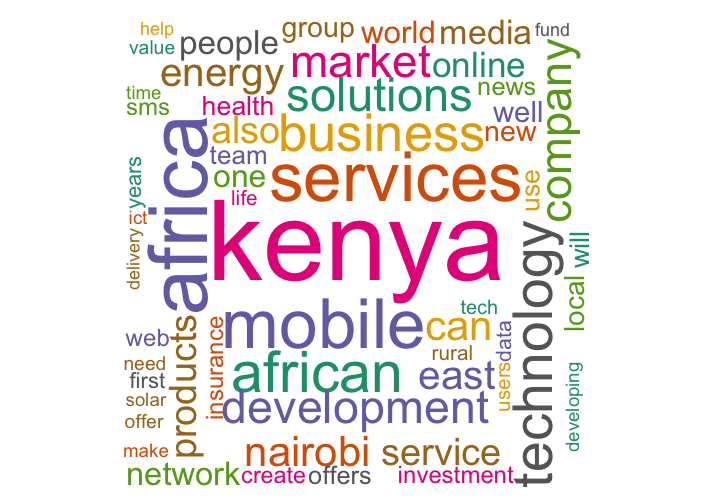
\includegraphics[scale=0.4]{kenya_cloud}
\caption{Word Cloud Generated from Kenyan Startups}
\end{figure}

If it is possible for ventures to position themselves deliberately along the continuum from social impact to profits-oriented, by means of marketing cues, are there funding-related advantages to presenting in a particular way? What are the language cues that most strongly indicate this orientation, and are there relationships between these cues and the amount, type and source of funding? 

I seek to answer these questions through a unique application of text analysis tools, employing supervised and unsupervised methods to understand linguistic features associated with social entrepreneurship, and then examining the relationship between these features and funding outcomes. This analysis was inspired in part by interviews with entrepreneurs in Lagos, Nigeria, the largest city in Africa and an emerging center for technology entrepreneurship.


\section{Theoretical Grounding}

The idea that organizations might deliberately manipulate their image for a given audience is rooted in the theories of impression management. Originally conceptualized as an individual-level psychological process, impression management refers to a number of behaviors that an individual might employ to influence how they are perceived by others (Bolino, Kacmar et al. 2008). This theory has subsequently been expanded to apply to organizations, referring to the tactics used by these organizations to burnish corporate reputations, control their image, or increase respectability (Highhouse, Brooks et al. 2009).

A substream of this literature refers specifically to impression management tactics employed by new ventures, who suffer from the much-cited ``liability of newness" (Yang and Aldrich 2011). This literature emphasizes that new ventures may strategically draw on impression management in order to secure resources from a variety of stakeholders. This process is not accidental: ``Entrepreneurs must be skilled cultural operators who shape interpretations of the nature and potential of their new venture to those who may supply needed resources" (Lounsbury and Glynn 2001). The way in which ventures choose to craft their image will depend on the institutional environment and normative beliefs of the potential audience (Zott and Huy 2007). Entrepreneurs, then, in this view, strategically assess how they can best fit into the preconceived mentality of the resource holders, and will shape their stories accordingly.

\begin{figure} [!h]
\centering
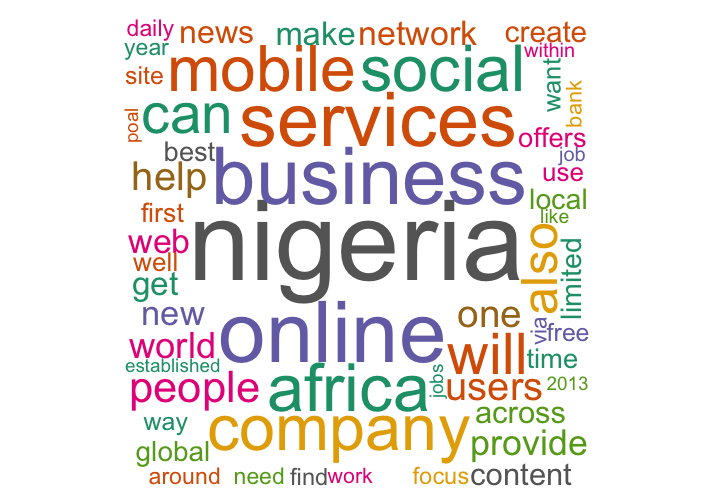
\includegraphics[scale=0.4]{nigeria_cloud}
\caption{Word Cloud Generated from Nigerian Startups}
\end{figure}

Most funding for ventures based in sub-Saharan Africa comes from foreign investors based in the US or Europe (Carstens 2013), who may bring a particular set of biases and beliefs to the table. Because of the continent’s unique baggage and its synonymy in the Western mind with poverty and dysfunction, it is likely that investors feel pressure to present their investments in a particular way. Describing the technology ecosystem in Kenya, Eleanor Marchant attributes the prevalence of social impact language to ``the legacy of the dominant aid discourse that permeates much ICT for development work in Africa, as well as the more recent ways in which multinational tech companies view their purpose in the country…such large economic actors might have a difficult time justifying their participation in the ecosystem without referring in some way to ‘social impact’" (2015).

This strategy can be seen reflected in the language used by venture capital firms active in the region. While the primary focus of these funds is profitable returns, positive social impact is often mentioned in the same breath. As an example, Netherlands-based eVA Fund notes that their purpose is ``investing capital and knowledge to strengthen small and medium sized internet related enterprises thus securing and creating jobs and income for large African communities and with that, generating attractive financial returns for investors" (2016). Novastar Ventures stresses that they are ``in search of businesses where positive social impact for lower-income households is a result of commercial success, not an end in itself" (2016). 

Ventures that mirror this type of language might then be attractive to these potential funding sources -- to a degree. As the director of an incubator in Lagos told this author, regarding venture capitalists and social impact: ``Sure, they care, but they don’t really care." It seems, then, that paying lip service to social impact may be helpful in attracting funding, but is by no means a substitute for a strong profit-generating business model. This would suggest that the best funding outcomes are achieved by startups that employ both types of language in their company marketing. 

The idea that firms that span the boundary between commercial and social goals may be most successful in attracting funding runs counter to main thesis of categorization theory, which suggests that firms or products that span multiple categories are disadvantaged (Hsu, Hannan et al. 2009). A possible explanation for this is that boundary spanning in mission (profit versus social goals) is fundamentally different from boundary spanning across industries or product categories. Indeed, the idea of a dual mission is part of the fundamental appeal of social entrepreneurship: essentially, the notion that you can have your cake and eat it too. It is also likely that this particular effect is specific to the developing country context and may not be present in rich economies.

It is also important to note that while acquiring funding is crucial to these small firms’ success, this is only one metric that is correlated with, but not entirely representative of, a firm’s performance. Particularly because most of the firms in this sample have only one round of seed funding, this metric represents more of a ``gut level" indicator of success that may or may not correspond with viable growth. It is likely that this commercial-social orientation may matter less for acquiring subsequent rounds of funding, as actual financial performance will become more important for securing further support. This is a question that I would like to investigate further, as the technology sector in sub-Saharan Africa continues to grow and more data becomes available.

\section{Methodology and Hypotheses}

To understand and track how entrepreneurs present themselves, the data for the text analysis is taken from Crunchbase, a global platform with detailed data on startups. Using this platform, I created a sample of 844 startups in sub-Saharan Africa (across Kenya, Nigeria, Uganda and Ghana). Each company provides a description of roughly one or two paragraphs to describe their activities, and the primary purpose of the platform is to generate exposure to potential funding sources. Figures 1 and 2 show word clouds created from the descriptions of startups based in Kenya and Nigeria. 

The first approach taken to understand the relationship between language and social entrepreneurship is a supervised one, leveraging the Mechanical Turk (mTurk) platform to recruit subjects to label the firms as either social entrepreneurship or not based on their descriptions. This type of crowdsourcing approach to annotating data is well established in sentiment analysis and other natural language tasks (Snow, O'Connor et al. 2008). Each rater was asked to read the descriptions of 30 firms and give a rating of zero (``not social entrepreneurship") or one (``social entrepreneurship"). By averaging across all raters, I generate a score for each firm between that ranges between zero and one, from most to least social.  

The second approach is unsupervised and provides a complimentary method of assessing the social orientation of the firms. I employed Latent Dirichlet allocation (LDA), a well-known generative topic model, to discover topic distributions across the startups’ descriptions (Blei, Ng et al. 2003). By finding the most stable topic model and labeling the resulting topics, I computed the relative proportions of the social impact topics and the profit-related topics within each firm’s description. These proportions serve as a measure of the social orientation of the firm that can be validated against the mTurk ratings.

The initial conjecture discussed above lends itself to the following two related hypotheses:

\textit{Hypothesis 1: Firms with greater mTurk rater disagreement on whether or not they constitute social entrepreneurship will have better funding outcomes.}

\textit{Hypothesis 2: Firms with high proportions of both social impact topics and profit-related topics in their descriptions, based on the LDA model, will have better funding outcomes.}

These measures of social orientation should be closely related, and similar results across both methods of measuring the independent variable should add strength to the argument that startups that emphasize both their profitability and their potential for social impact will achieve the greater success in attracting funding.


\section{Results: mTurk Scores and Funding}

To acquire external measures of the firms’ social orientations, social entrepreneurship was defined for the raters on mTurk as ``innovative, social value creating activity that can occur within or across the nonprofit, business or government sectors'' (Austin, Stevenson et al. 2006). Each rater was given 30 companies to rate, and quality checks were inserted to insure that they were reading carefully. Ultimately, each firm was rated by an average of between 15 and 16 mTurk users. The resulting ``mTurk Score'' for a particular firm is the mean of all these users’ ratings, ranging from zero (if all users agreed that firm did not constitute social entrepreneurship) to one (if all users agreed that it did). Across the firms, the mean mTurk Score was 0.44, with a standard deviation of 0.21. 

As a check on whether the users understood the task, Table 1 shows the words selected by a Lasso regression of the mTurk Score on the words in the companies’ descriptions. \footnote{This model treats each description as a sparse document-term matrix, in which the covariates are each word in the vocabulary and the values are the count of times those words appear in the description. Regularization via the Lasso adds a penalization term (proportional to the sum of the absolute values of the coefficients) to the optimization process (Tibshirani 1996). A shrinkage parameter $\lambda$ controls the extent of the regularization (when $\lambda$ is equal to zero, the results are identical to OLS). Because of the nature of the absolute value term, Lasso produces sparse coefficient vectors, which is highly useful in this case due to the number of terms in the vocabulary.  The optimal level of the shrinkage parameter was selected via cross-validation with ten folds, choosing the model that minimized mean squared error.} The words are ordered by the size of the coefficient, with the most negative coefficients being predictive of a lower, less social score, and the largest positive coefficients predicting a higher, more social score. The resulting model is highly intuitive, with words like ``poverty'', ``charity'', ``communities'', ``youth'' and ``schools'' having the largest coefficients, and the most negative coefficients belonging to words like ``immediately'', ``leading'', ``provider'', ``develops'', and ``branches''. Appendix Tables 1 and 2 display results from a similar process run only on the lower half and the upper half of the scores, respectively. This provides some insight into what type of language distinguishes low from middle scores, and middle from high scores.

\begin{minipage}{\textwidth}
\centering
\captionof{table}{Words Selected by LASSO model predicting mTurk score}
\begingroup\small
\pgfplotstabletypeset[
    every head row/.style={before row=\toprule,after row=\midrule},
    every last row/.style={after row=\bottomrule},
    col sep=ampersand,
    row sep=\\,
    %
    columns={Feature,Coefficient,Feature,Coefficient},
    display columns/0/.style={
        % first part of 2 of thing':
        select equal part entry of={0}{2},
        string type,
            % column display name:
        column name={Feature},
        column type={c}, % ... and type
    },
    display columns/1/.style={
        % first part of 2 of mapsto':
        select equal part entry of={0}{2},
        string type,
        column name={Coefficient},
        column type={l|},
    },
    display columns/2/.style={select equal part entry of={1}{2},string type},% second part of 2 of thing'
    display columns/3/.style={select equal part entry of={1}{2},string type},% second part of 2 of maps'
]{
    Feature & Coefficient \\
    immediately & -0.03 \\ 
  leading & -0.02 \\ 
  provider & -0.02 \\ 
  develops & -0.02 \\ 
  branches & -0.01 \\ 
  nairobi & -0.01 \\ 
  email & -0.01 \\ 
  firm & -0.01 \\ 
  company & -0.01 \\ 
  securities & -0.01 \\ 
  delivery & -0.01 \\ 
  management & -0.01 \\ 
  agency & -0.01 \\ 
  strong & -0.01 \\ 
  exchange & -0.01 \\ 
  limited & -0.01 \\ 
  telecommunication & -0.00 \\ 
  eastern & -0.00 \\ 
  bank & -0.00 \\ 
  solution & -0.00 \\ 
  web & -0.00 \\ 
  online & -0.00 \\ 
  subsidiary & -0.00 \\ 
  water & 0.00 \\ 
  enough & 0.00 \\ 
  give & 0.00 \\ 
  mentoring & 0.00 \\ 
  job & 0.00 \\ 
  solar & 0.00 \\ 
  share & 0.00 \\ 
  foundation & 0.00 \\ 
  pool & 0.01 \\ 
  materials & 0.01 \\ 
  study & 0.01 \\ 
  better & 0.01 \\ 
  interact & 0.01 \\ 
  opportunity & 0.01 \\ 
  discover & 0.01 \\ 
  incubator & 0.01 \\ 
  education & 0.01 \\ 
  leveraging & 0.01 \\ 
  care & 0.01 \\ 
  supporting & 0.01 \\ 
  rural & 0.01 \\ 
  forum & 0.01 \\ 
  solving & 0.01 \\ 
  start-up & 0.01 \\ 
  entrepreneurs & 0.01 \\ 
  hub & 0.01 \\ 
  children & 0.01 \\ 
  directions & 0.01 \\ 
  sustainability & 0.02 \\ 
  accessibility & 0.02 \\ 
  programs & 0.02 \\ 
  patients & 0.02 \\ 
  together & 0.02 \\ 
  entrepreneurship & 0.02 \\ 
  healthcare & 0.02 \\ 
  create & 0.02 \\ 
  improve & 0.02 \\ 
  clean & 0.02 \\ 
  affordable & 0.02 \\ 
  solve & 0.02 \\ 
  access & 0.02 \\ 
  women & 0.02 \\ 
  farmers & 0.03 \\ 
  urban & 0.03 \\ 
  raise & 0.03 \\ 
  health & 0.03 \\ 
  teach & 0.03 \\ 
  non-profit & 0.03 \\ 
  enhancing & 0.03 \\ 
  awareness & 0.03 \\ 
  social & 0.03 \\ 
  scale & 0.03 \\ 
  lives & 0.03 \\ 
  people & 0.04 \\ 
  community & 0.04 \\ 
  educational & 0.04 \\ 
  civil & 0.04 \\ 
  sustainable & 0.05 \\ 
  africans & 0.05 \\ 
  households & 0.05 \\ 
  students & 0.06 \\ 
  schools & 0.06 \\ 
  youth & 0.07 \\ 
  communities & 0.08 \\ 
  charity & 0.10 \\ 
  poverty & 0.10 \\ 
  (Intercept) & 0.40 \\ 
}
\endgroup
\end{minipage}


Hypothesis 1 predicted that firms with more user disagreement over whether or not they constituted social entrepreneurship -- that is, scores in the middle of the range -- would have better funding outcomes than those on either extreme. Figure 3 displays the proportion of firms funded at each range of the mTurk Score. An inverted-U pattern is clearly evident, with the peak appearing to be slightly toward the less-social part of the spectrum. Table 2 shows evidence for this same effect, with a logistic regression of the funding indicator run on a quadratic model of the mTurk Score. This effect persists even when controlling for country (Model 1), for the four most common industries (Model 2), and for all industry fixed effects (Model 3). 

\begin{figure} [!htb]
\centering
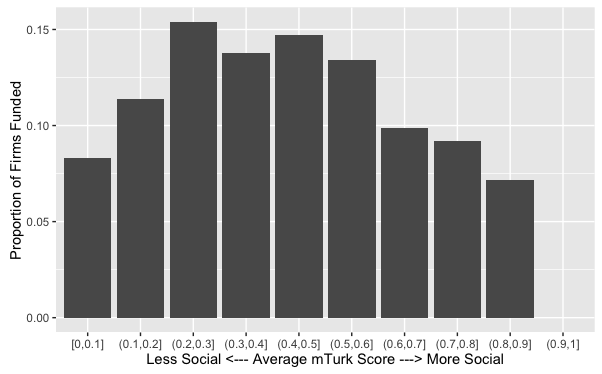
\includegraphics[scale=0.55]{proportion_funded}
\caption{Proportion of Firms Funded by mTurk Score}
\end{figure}

% Table created by stargazer v.5.2 by Marek Hlavac, Harvard University. E-mail: hlavac at fas.harvard.edu
% Date and time: Fri, Jun 24, 2016 - 13:36:08
\begin{table}[!htbp] \centering 
  \caption{Logistic Regression of Funding Dummy on mTurk Score} 
  \label{} 
\footnotesize
\begin{tabular}{@{\extracolsep{5pt}}lccc} 
\\[-1.8ex]\hline 
\hline \\[-1.8ex] 
 & \multicolumn{3}{c}{Funding indicator} \\ 
\cline{2-4} 
\\[-1.8ex] & \multicolumn{3}{c}{} \\ 
 & Model 1 & Model 2 & Model 3 \\ 
\\[-1.8ex] & (1) & (2) & (3)\\ 
\hline \\[-1.8ex] 
 mTurk Score & 4.37$^{*}$ & 4.82$^{*}$ & 7.46$^{**}$ \\ 
  & (2.55) & (2.65) & (3.74) \\ 
  mTurk Score*2 & $-$5.17$^{*}$ & $-$5.27$^{*}$ & $-$7.75$^{*}$ \\ 
  & (2.69) & (2.78) & (3.98) \\ 
  Kenya & $-$0.03 & 0.14 & 0.49 \\ 
  & (0.37) & (0.38) & (0.57) \\ 
  Nigeria & 0.14 & 0.24 & 0.81 \\ 
  & (0.36) & (0.37) & (0.56) \\ 
  Uganda & 0.45 & 0.53 & 0.72 \\ 
  & (0.44) & (0.45) & (0.69) \\ 
  Software &  & 1.01$^{***}$ & 2.03$^{***}$ \\ 
  &  & (0.34) & (0.50) \\ 
  Mobile &  & 0.82$^{**}$ & 0.30 \\ 
  &  & (0.33) & (0.65) \\ 
  E-Commerce &  & 0.73$^{*}$ & 1.28$^{**}$ \\ 
  &  & (0.38) & (0.56) \\ 
  Education &  & 0.59 & 1.85$^{***}$ \\ 
  &  & (0.44) & (0.62) \\ 
  Constant & $-$2.84$^{***}$ & $-$3.40$^{***}$ & $-$5.66$^{***}$ \\ 
  & (0.64) & (0.69) & (1.05) \\ 
 \hline \\[-1.8ex] 
 All 200+ Industries & No & No & Yes  \\ 
 \hline \\[-1.8ex] 
Observations & 844 & 844 & 844 \\ 
\hline 
\hline \\[-1.8ex] 
\textit{Note:}  & \multicolumn{3}{r}{$^{*}$p$<$0.1; $^{**}$p$<$0.05; $^{***}$p$<$0.01} \\ 
\end{tabular} 
\end{table} 

Because this sample consists of primarily early-stage African startups, most of which have no external funding, the funding indicator is the most useful outcome variable for this analysis. However, it is useful to see whether any particular type of funding drives the observed effect. Table 3 displays logistic regression models for various different funding indicators. The quadratic effect discussed above can be observed for firms acquiring their first funding round, but does not appear to predict subsequent funding rounds (although there may not be enough data to demonstrate this effect, as only a minority of firms have more than one funding round). Similarly, there appears to be a borderline significant quadratic effect for acquiring seed funding, but not for venture or private equity funding. Ideally, follow-up research with access to a larger sample of funded firms would plumb these contradictions further. However, it may be that spanning the commercial-social boundary is most crucial for acquiring early stage funding, and this orientation matters less for subsequent funding acquisition. 


% Table created by stargazer v.5.2 by Marek Hlavac, Harvard University. E-mail: hlavac at fas.harvard.edu
% Date and time: Thu, Jun 23, 2016 - 19:49:24
\begin{table}[!htbp] \centering 
  \caption{Specific Types of Funding Outcomes} 
  \label{} 
\footnotesize 
\begin{tabular}{@{\extracolsep{5pt}}lcccc} 
\\[-1.8ex]\hline 
\hline \\[-1.8ex] 
 & \multicolumn{4}{c}{Funding Indicators} \\ 
\cline{2-5} 
\\[-1.8ex] &  &  &  &  \\ 
 & First Funding Round & Subsequent Funding Rounds & Seed Funding & Venture/PE Funding \\ 
\\[-1.8ex] & (1) & (2) & (3) & (4)\\ 
\hline \\[-1.8ex] 
 mTurk Score & 8.58$^{**}$ & $-$10.48 & 8.40$^{*}$ & 0.18 \\ 
  & (3.98) & (14.49) & (4.40) & (8.18) \\ 
  mTurk Score*2 & $-$8.67$^{**}$ & 6.72 & $-$7.30 & $-$0.38 \\ 
  & (4.20) & (18.75) & (4.48) & (9.24) \\ 
  Kenya & 0.68 & $-$3.19$^{**}$ & 0.01 & 1.93 \\ 
  & (0.64) & (1.58) & (0.56) & (1.46) \\ 
  Nigeria & 1.14$^{*}$ & $-$4.72$^{**}$ & $-$0.49 & 1.01 \\ 
  & (0.61) & (2.17) & (0.58) & (1.46) \\ 
  Uganda & 0.74 & $-$0.51 & $-$0.11 & 0.69 \\ 
  & (0.77) & (2.19) & (0.70) & (1.96) \\ 
  Constant & $-$6.33$^{***}$ & $-$2.57 & $-$5.30$^{***}$ & $-$5.35$^{**}$ \\ 
  & (1.14) & (2.90) & (1.20) & (2.17) \\ 
 \hline \\[-1.8ex] 
 All 200+ Industries & Yes & Yes & Yes & Yes \\ 
  \hline \\[-1.8ex] 
Observations & 824 & 844 & 844 & 844 \\ 
\hline 
\hline \\[-1.8ex] 
\textit{Note:}  & \multicolumn{4}{r}{$^{*}$p$<$0.1; $^{**}$p$<$0.05; $^{***}$p$<$0.01} \\ 
\end{tabular} 
\end{table} 

\FloatBarrier

\section{Results: Topics}


\begin{figure} [!h]
\centering
\includegraphics[scale=0.9]{Topics}
\caption{Top Words from Each Topic}
\end{figure}

\begin{figure} [!htb]
\centering
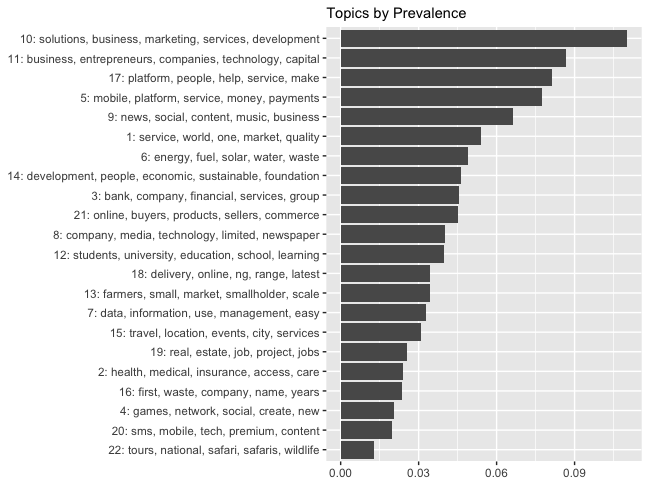
\includegraphics[scale=0.6]{topic_prevalence}
\caption{Topics Sorted by Estimated Prevalence in Company Descriptions}
\end{figure}

\begin{figure} [!htb]
\centering
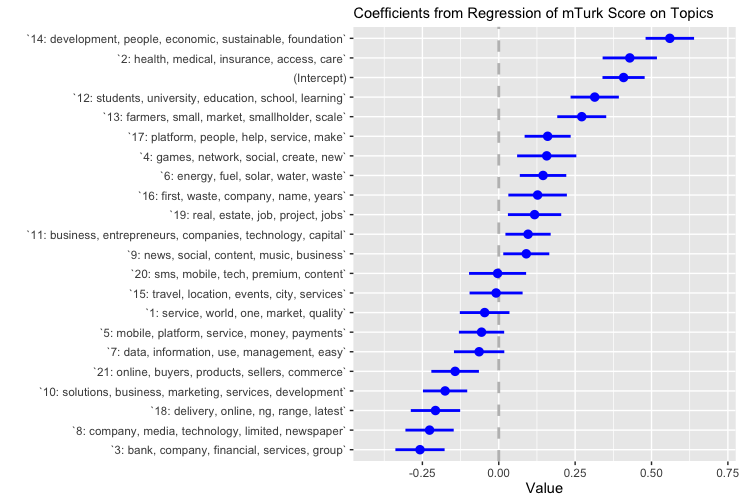
\includegraphics[scale=0.6]{topics_coefplot}
\caption{Topics Sorted by Relationship with mTurk Score (most to least social)}
\end{figure}

% Table created by stargazer v.5.2 by Marek Hlavac, Harvard University. E-mail: hlavac at fas.harvard.edu
% Date and time: Thu, Jun 23, 2016 - 20:39:32
\begin{table}[!htbp] \centering 
  \caption{Logistic Regression of Funding Dummy on Topic-mTurk Score Interaction} 
  \label{} 
\footnotesize 
\begin{tabular}{@{\extracolsep{5pt}}lcc} 
\\[-1.8ex]\hline 
\hline \\[-1.8ex] 
 & \multicolumn{2}{c}{Funding Indicator} \\ 
\cline{2-3} 
\\[-1.8ex] & \multicolumn{2}{c}{} \\ 
 & Model 1 & Model 2 \\ 
\\[-1.8ex] & (1) & (2)\\ 
\hline \\[-1.8ex] 
 T1: quality & $-$2.83 (1.88) & $-$4.87 (5.15) \\ 
  T2: health & $-$2.33 (2.17) & $-$7.72 (8.41) \\ 
  T3: banking & $-$4.95$^{**}$ (2.50) & $-$14.55$^{**}$ (7.26) \\ 
  T4: gaming/networks & $-$0.10 (1.84) & $-$5.43 (5.67) \\ 
  T5: mobile platforms & $-$1.34 (1.51) & $-$6.52 (4.64) \\ 
  T6: energy & $-$0.51 (1.50) & $-$4.56 (4.68) \\ 
  T7: data & $-$1.12 (1.70) & $-$8.75$^{*}$ (5.29) \\ 
  T8: media & 0.42 (1.49) & $-$4.31 (4.36) \\ 
  T9: content & $-$0.05 (1.46) & $-$5.88 (4.62) \\ 
  T10: business solutions & 0.25 (1.40) & $-$7.13$^{*}$ (4.33) \\ 
  T11: entrepreneurship & $-$0.59 (1.46) & $-$3.61 (4.41) \\ 
  T12: education & $-$0.09 (1.52) & $-$1.17 (4.81) \\ 
  T13: farming & $-$1.02 (1.67) & $-$8.24 (5.96) \\ 
  T14: development/non-profit & $-$0.14 (1.56) & $-$8.90 (6.24) \\ 
  T15: events & 0.22 (1.64) & $-$7.84 (5.06) \\ 
  T16: time & $-$3.38 (2.47) & $-$5.63 (6.20) \\ 
  T17: service & $-$0.24 (1.46) & $-$1.96 (4.60) \\ 
  T18: delivery & $-$0.79 (1.64) & $-$10.53$^{**}$ (5.15) \\ 
  T19: real estate & 0.21 (1.65) & $-$5.15 (4.91) \\ 
  T20: SMS & $-$0.38 (1.80) & $-$2.50 (4.79) \\ 
  T21: e-commerce & $-$1.51 (1.66) & $-$6.01 (4.76) \\ 
  Score x T1: quality &  & $-$7.99 (7.63) \\ 
  Score x T2: health &  & 0.22 (10.80) \\ 
  Score x T3: banking &  & 12.45 (11.55) \\ 
  Score x T4: gaming/networks &  & 0.15 (7.23) \\ 
  Score x T5: mobile platforms &  & 0.46 (4.72) \\ 
  Score x T6: energy &  & $-$2.08 (3.72) \\ 
  Score x T7: data &  & 6.52 (6.95) \\ 
  Score x T8: media &  & $-$1.41 (4.10) \\ 
  Score x T9: content &  & 1.96 (3.50) \\ 
  \textbf{Score x T10: business solutions} &  & \textbf{7.82}$^{***}$ (2.81) \\ 
  Score x T11: entrepreneurship &  & $-$4.46 (2.94) \\ 
  \textbf{Score x T12: education} &  & $-$ \textbf{7.59}$^{*}$ (4.36) \\ 
  Score x T13: farming &  & 3.47 (6.47) \\ 
  Score x T14: development/non-profit &  & 5.19 (6.14) \\ 
  Score x T15: events &  & 6.15 (5.67) \\ 
  Score x T16: time &  & $-$6.27 (10.10) \\ 
  \textbf{Score x T17: service} &  & $-$ \textbf{7.02}$^{*}$ (3.91) \\ 
  \textbf{Score x T18: delivery} &  &  \textbf{13.90}$^{**}$ (7.08) \\ 
  Score x T19: real estate &  & 0.53 (5.39) \\ 
  Score x T20: SMS &  & $-$7.69 (6.21) \\ 
  Score x T21: e-commerce &  & $-$1.85 (6.08) \\ 
  Score x T22: safaris &  & $-$13.62 (12.44) \\ 
  Kenya & $-$0.11 (0.38) & $-$0.12 (0.40) \\ 
  Nigeria & 0.03 (0.37) & 0.04 (0.39) \\ 
  Uganda & 0.18 (0.45) & 0.24 (0.48) \\ 
  Constant & $-$1.37 (1.37) & 3.63 (4.18) \\ 
 \hline \\[-1.8ex] 
Observations & 844 & 844 \\ 
\hline 
\hline \\[-1.8ex] 
\textit{Note:}  & \multicolumn{2}{r}{$^{*}$p$<$0.1; $^{**}$p$<$0.05; $^{***}$p$<$0.01} \\ 
\end{tabular} 
\end{table} 

% Table created by stargazer v.5.2 by Marek Hlavac, Harvard University. E-mail: hlavac at fas.harvard.edu
% Date and time: Fri, Jun 24, 2016 - 13:26:19
\begin{table}[!htbp] \centering 
  \caption{Interactions with Banking Topic} 
  \label{} 
\footnotesize 
\begin{tabular}{@{\extracolsep{5pt}}lcc} 
\\[-1.8ex]\hline 
\hline \\[-1.8ex] 
 & \multicolumn{2}{c}{Funding Indicator} \\ 
\cline{2-3} 
\\[-1.8ex] & \multicolumn{2}{c}{} \\ 
\\[-1.8ex] & (1) & (2)\\ 
\hline \\[-1.8ex] 
  T3: banking & $-$4.95$^{**}$ & $-$137.99$^{*}$ \\ 
  & (2.50) & (73.29) \\ 
  T3 x T1: quality &  & 156.66$^{*}$ \\ 
  &  & (93.64) \\ 
  T3 x T5: mobile platforms &  & 165.38$^{*}$ \\ 
  &  & (91.92) \\ 
  \textbf{T3 x T6: energy} &  & \textbf{209.25}$^{**}$ \\ 
  &  & (97.88) \\ 
  T3 x T8: media &  & 224.72$^{**}$ \\ 
  &  & (111.20) \\ 
  T3 x T9: content &  & 174.20$^{*}$ \\ 
  &  & (92.83) \\ 
  T3 x T11: entrepreneurship &  & 162.26$^{*}$ \\ 
  &  & (86.09) \\ 
  \textbf{T3 x T12: education} &  & \textbf{243.36}$^{**}$ \\ 
  &  & (112.34) \\ 
  \textbf{T3 x T13: farming} &  & \textbf{236.77}$^{**}$ \\ 
  &  & (113.92) \\ 
  \textbf{T3 x T14: development/non-profit} &  & \textbf{130.53}$^{*}$ \\ 
  &  & (74.01) \\ 
  T3 x T19: real estate &  & 231.65$^{*}$ \\ 
  &  & (126.10) \\ 
  Kenya & $-$0.11 & $-$0.02 \\ 
  & (0.38) & (0.40) \\ 
  Nigeria & 0.03 & 0.15 \\ 
  & (0.37) & (0.39) \\ 
  Uganda & 0.18 & 0.35 \\ 
  & (0.45) & (0.47) \\ 
  Constant & $-$1.37 & $-$0.49 \\ 
  & (1.37) & (1.45) \\ 
 \hline \\[-1.8ex] 
Observations & 844 & 844 \\ 
\hline 
\hline \\[-1.8ex] 
\multicolumn{3}{r}{$^{*}$p$<$0.1; $^{**}$p$<$0.05; $^{***}$p$<$0.01} \\ 
 \multicolumn{3}{r}{\scriptsize{All individual topics and interactions with T3 are included.}} \\ 
 \multicolumn{3}{r}{\scriptsize{Only significant interactions are displayed.}} \\ 
\end{tabular} 
\end{table} 

% Table created by stargazer v.5.2 by Marek Hlavac, Harvard University. E-mail: hlavac at fas.harvard.edu
% Date and time: Fri, Jun 24, 2016 - 13:31:33
\begin{table}[!htbp] \centering 
  \caption{Interactions with Development/Non-Profit Topic} 
  \label{} 
\footnotesize 
\begin{tabular}{@{\extracolsep{5pt}}lcc} 
\\[-1.8ex]\hline 
\hline \\[-1.8ex] 
 & \multicolumn{2}{c}{Funding Indicator} \\ 
\cline{2-3} 
\\[-1.8ex] & \multicolumn{2}{c}{} \\ 
\\[-1.8ex] & (1) & (2)\\ 
\hline \\[-1.8ex] 
  T14: development/non-profit & $-$0.14 & $-$3.88 \\ 
  & (1.56) & (3.17) \\ 
  T14 x T6: energy &  & 18.90$^{*}$ \\ 
  &  & (9.65) \\ 
  \textbf{T14 x T8: media} &  & \textbf{34.85}$^{**}$ \\ 
  &  & (17.08) \\ 
   \textbf{T14 x T9: content} &  & \textbf{47.06}$^{**}$ \\ 
  &  & (20.54) \\ 
  Kenya & $-$0.11 & $-$0.13 \\ 
  & (0.38) & (0.40) \\ 
  Nigeria & 0.03 & 0.09 \\ 
  & (0.37) & (0.38) \\ 
  Uganda & 0.18 & 0.34 \\ 
  & (0.45) & (0.47) \\ 
  Constant & $-$1.37 & $-$1.37 \\ 
  & (1.37) & (1.45) \\ 
 \hline \\[-1.8ex] 
Observations & 844 & 844 \\ 
\hline 
\hline \\[-1.8ex] 
 \multicolumn{3}{r}{$^{*}$p$<$0.1; $^{**}$p$<$0.05; $^{***}$p$<$0.01} \\ 
 \multicolumn{3}{r}{ \scriptsize{All individual topics and interactions with T14 are included.}} \\ 
 \multicolumn{3}{r}{\scriptsize{Only significant interactions are displayed.}} \\ 
\end{tabular} 
\end{table} 


\section{Discussion and Conclusion}


\section{References}


\clearpage

\section{Appendix}

\setcounter{table}{0}
\renewcommand{\thetable}{A\arabic{table}}

\setcounter{figure}{0}
\renewcommand{\thefigure}{A\arabic{figure}}


\begin{minipage}{\textwidth}
\centering
\captionof{table}{Words that distinguish low from middle mTurk scores}
\begingroup\footnotesize
\pgfplotstabletypeset[
    every head row/.style={before row=\toprule,after row=\midrule},
    every last row/.style={after row=\bottomrule},
    col sep=ampersand,
    row sep=\\,
    %
    columns={Feature,Coefficient,Feature,Coefficient},
    display columns/0/.style={
        % first part of 2 of thing':
        select equal part entry of={0}{2},
        string type,
            % column display name:
        column name={Feature},
        column type={c}, % ... and type
    },
    display columns/1/.style={
        % first part of 2 of mapsto':
        select equal part entry of={0}{2},
        string type,
        column name={Coefficient},
        column type={l|},
    },
    display columns/2/.style={select equal part entry of={1}{2},string type},% second part of 2 of thing'
    display columns/3/.style={select equal part entry of={1}{2},string type},% second part of 2 of maps'
]{
    Feature & Coefficient \\
    firm & -0.64 \\ 
  price & -0.58 \\ 
  (Intercept) & -0.57 \\ 
  ltd & -0.42 \\ 
  solution & -0.41 \\ 
  booking & -0.40 \\ 
  analytics & -0.38 \\ 
  africa's & -0.36 \\ 
  record & -0.36 \\ 
  brand & -0.28 \\ 
  turn & -0.27 \\ 
  name & -0.23 \\ 
  nigeria's & -0.23 \\ 
  within & -0.21 \\ 
  post & -0.19 \\ 
  organisation & -0.17 \\ 
  management & -0.15 \\ 
  states & -0.14 \\ 
  headquartered & -0.14 \\ 
  bank & -0.11 \\ 
  banking & -0.10 \\ 
  mobility & -0.09 \\ 
  sale & -0.08 \\ 
  kingdom & -0.07 \\ 
  goods & -0.06 \\ 
  provider & -0.04 \\ 
  always & -0.04 \\ 
  using & 0.02 \\ 
  school & 0.03 \\ 
  potential & 0.03 \\ 
  unlike & 0.04 \\ 
  family & 0.04 \\ 
  government & 0.04 \\ 
  enhancing & 0.05 \\ 
  sustainable & 0.05 \\ 
  investment & 0.05 \\ 
  enable & 0.05 \\ 
  source & 0.06 \\ 
  long & 0.07 \\ 
  videos & 0.09 \\ 
  lifestyle & 0.09 \\ 
  income & 0.09 \\ 
  material & 0.11 \\ 
  manage & 0.11 \\ 
  portal & 0.12 \\ 
  provide & 0.12 \\ 
  formed & 0.13 \\ 
  extra & 0.13 \\ 
  daily & 0.13 \\ 
  local & 0.14 \\ 
  europe & 0.15 \\ 
  classes & 0.15 \\ 
  language & 0.15 \\ 
  users & 0.16 \\ 
  africa & 0.17 \\ 
  startups & 0.17 \\ 
  employers & 0.18 \\ 
  send & 0.19 \\ 
  helps & 0.20 \\ 
  seed & 0.20 \\ 
  whole & 0.20 \\ 
  promote & 0.22 \\ 
  ideal & 0.23 \\ 
  major & 0.23 \\ 
  university & 0.23 \\ 
  initiative & 0.24 \\ 
  energy & 0.24 \\ 
  small & 0.25 \\ 
  model & 0.26 \\ 
  public & 0.27 \\ 
  free & 0.28 \\ 
  financing & 0.32 \\ 
  unlimited & 0.33 \\ 
  african & 0.33 \\ 
  cook & 0.34 \\ 
  open & 0.34 \\ 
  founders & 0.39 \\ 
  take & 0.39 \\ 
  realized & 0.39 \\ 
  june & 0.42 \\ 
  members & 0.45 \\ 
  used & 0.45 \\ 
  text & 0.45 \\ 
  activities & 0.48 \\ 
  hot & 0.50 \\ 
  favorite & 0.51 \\ 
  platform & 0.51 \\ 
  social & 0.53 \\ 
  places & 0.55 \\ 
  annually & 0.57 \\ 
  export & 0.58 \\ 
  news & 0.59 \\ 
  countries & 0.63 \\ 
  b2b & 0.63 \\ 
  improvement & 0.64 \\ 
  people & 0.68 \\ 
  event & 0.71 \\ 
  established & 0.78 \\ 
  spend & 0.79 \\ 
  around & 0.80 \\ 
  relevant & 0.81 \\ 
  territory & 0.82 \\ 
  channels & 1.37 \\ 
}
\endgroup
\end{minipage}


\newpage

\begin{minipage}{\textwidth}
\centering
\captionof{table}{Words that distinguish middle from high mTurk scores}
\begingroup\footnotesize
\pgfplotstabletypeset[
    every head row/.style={before row=\toprule,after row=\midrule},
    every last row/.style={after row=\bottomrule},
    col sep=ampersand,
    row sep=\\,
    %
    columns={Feature,Coefficient,Feature,Coefficient},
    display columns/0/.style={
        % first part of 2 of thing':
        select equal part entry of={0}{2},
        string type,
            % column display name:
        column name={Feature},
        column type={c}, % ... and type
    },
    display columns/1/.style={
        % first part of 2 of mapsto':
        select equal part entry of={0}{2},
        string type,
        column name={Coefficient},
        column type={l|},
    },
    display columns/2/.style={select equal part entry of={1}{2},string type},% second part of 2 of thing'
    display columns/3/.style={select equal part entry of={1}{2},string type},% second part of 2 of maps'
]{
    Feature & Coefficient \\
    engineering & -0.67 \\ 
  whole & -0.57 \\ 
  app & -0.45 \\ 
  user & -0.45 \\ 
  investment & -0.40 \\ 
  software & -0.39 \\ 
  ideal & -0.39 \\ 
  leading & -0.39 \\ 
  enable & -0.38 \\ 
  seamless & -0.36 \\ 
  customers & -0.36 \\ 
  (Intercept) & -0.35 \\ 
  sell & -0.35 \\ 
  entertainment & -0.31 \\ 
  places & -0.31 \\ 
  manage & -0.31 \\ 
  unlimited & -0.31 \\ 
  word & -0.30 \\ 
  fashion & -0.30 \\ 
  capital & -0.27 \\ 
  general & -0.26 \\ 
  product & -0.25 \\ 
  google & -0.24 \\ 
  clients & -0.24 \\ 
  analysis & -0.24 \\ 
  media & -0.21 \\ 
  magazine & -0.20 \\ 
  sellers & -0.18 \\ 
  company & -0.17 \\ 
  companies & -0.17 \\ 
  news & -0.17 \\ 
  investor & -0.16 \\ 
  generate & -0.16 \\ 
  government & -0.15 \\ 
  started & -0.15 \\ 
  owned & -0.15 \\ 
  regulatory & -0.14 \\ 
  territory & -0.12 \\ 
  transactions & -0.10 \\ 
  reviews & -0.09 \\ 
  nairobi & -0.09 \\ 
  money & -0.09 \\ 
  strategy & -0.09 \\ 
  wallet & -0.07 \\ 
  base & -0.07 \\ 
  required & -0.06 \\ 
  african & -0.04 \\ 
  shopping & -0.04 \\ 
  hot & -0.02 \\ 
  internet & -0.02 \\ 
  advertising & -0.01 \\ 
  stories & -0.00 \\ 
  service & -0.00 \\ 
  non-profit & 0.01 \\ 
  child & 0.01 \\ 
  answers & 0.02 \\ 
  environment & 0.03 \\ 
  connect & 0.03 \\ 
  another & 0.04 \\ 
  ideas & 0.04 \\ 
  women & 0.04 \\ 
  solving & 0.07 \\ 
  post & 0.08 \\ 
  improved & 0.08 \\ 
  life & 0.09 \\ 
  africans & 0.10 \\ 
  people & 0.10 \\ 
  organisation & 0.10 \\ 
  booking & 0.11 \\ 
  waste & 0.11 \\ 
  awareness & 0.12 \\ 
  economic & 0.13 \\ 
  start-up & 0.13 \\ 
  towards & 0.13 \\ 
  urban & 0.13 \\ 
  united & 0.16 \\ 
  farmers & 0.16 \\ 
  feed & 0.18 \\ 
  education & 0.18 \\ 
  scale & 0.18 \\ 
  recruitment & 0.20 \\ 
  households & 0.22 \\ 
  mission & 0.23 \\ 
  lives & 0.23 \\ 
  price & 0.24 \\ 
  social & 0.24 \\ 
  healthcare & 0.24 \\ 
  pool & 0.25 \\ 
  patients & 0.26 \\ 
  health & 0.26 \\ 
  study & 0.27 \\ 
  share & 0.28 \\ 
  access & 0.29 \\ 
  sells & 0.30 \\ 
  improve & 0.31 \\ 
  entrepreneurship & 0.31 \\ 
  networking & 0.32 \\ 
  supported & 0.33 \\ 
  raise & 0.34 \\ 
  interests & 0.35 \\ 
  foundation & 0.40 \\ 
  problems & 0.46 \\ 
  enhance & 0.46 \\ 
  affordable & 0.51 \\ 
  students & 0.52 \\ 
  strive & 0.53 \\ 
  charity & 0.64 \\ 
  educational & 0.66 \\ 
  youth & 0.74 \\ 
  informal & 0.79 \\ 
  teach & 0.85 \\ 
  poverty & 0.90 \\ 
  communities & 0.96 \\ 
}
\endgroup
\end{minipage}


\begin{figure} [!h]
\centering
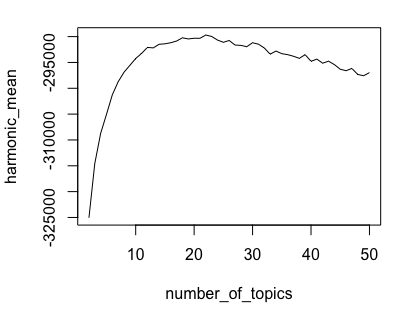
\includegraphics[scale=0.6]{harmonic_mean}
\caption{Maximization of Harmonic Mean for Topic Number Selection}
\end{figure}


% Table created by stargazer v.5.2 by Marek Hlavac, Harvard University. E-mail: hlavac at fas.harvard.edu
% Date and time: Thu, Jun 23, 2016 - 16:11:41
\begin{table}[!htbp] \centering 
  \caption{Regressions of Total Funding on mTurk Score} 
  \label{} 
\footnotesize 
\begin{tabular}{@{\extracolsep{5pt}}lcccccc} 
\\[-1.8ex]\hline 
\hline \\[-1.8ex] 
 & \multicolumn{6}{c}{Funding Amount: Less than...} \\ 
\cline{2-7} 
\\[-1.8ex] & \multicolumn{6}{c}{} \\ 
 & \textdollar 10m &  \textdollar 1m &  \textdollar 400k &  \textdollar 200k &  \textdollar 50k &  \textdollar 25k \\ 
\\[-1.8ex] & (1) & (2) & (3) & (4) & (5) & (6)\\ 
\hline \\[-1.8ex] 
 mTurk Score & 188,883 & 21,205 & 43,249$^{**}$ & 24,880$^{*}$ & 2,031 & 2,048 \\ 
  & (340,299) & (44,280) & (20,577) & (13,101) & (3,169) & (1,908) \\ 
  mTurk Score*2 & $-$150,817 & $-$16,363 & $-$39,834$^{*}$ & $-$26,372$^{*}$ & $-$1,459 & $-$1,676 \\ 
  & (354,938) & (46,167) & (21,436) & (13,642) & (3,298) & (1,984) \\ 
  Kenya & 61,072 & $-$5,430 & $-$4,817 & $-$1,573 & $-$72 & 310 \\ 
  & (53,155) & (6,979) & (3,259) & (2,074) & (507) & (306) \\ 
  Nigeria & 50,273 & $-$11,617$^{*}$ & $-$2,791 & $-$706 & 34 & 268 \\ 
  & (52,802) & (6,920) & (3,228) & (2,056) & (501) & (304) \\ 
  Uganda & 32,511 & $-$12,483 & $-$6,135 & $-$282 & 174 & 957$^{**}$ \\ 
  & (69,215) & (9,075) & (4,236) & (2,697) & (658) & (397) \\ 
  Constant & $-$46,310 & 4,573 & $-$6,770 & $-$3,648 & $-$434 & $-$883$^{*}$ \\ 
  & (88,906) & (11,558) & (5,393) & (3,429) & (831) & (501) \\ 
   \hline \\[-1.8ex] 
 All 200+ Industries & Yes & Yes & Yes & Yes & Yes & Yes\\ 
 \hline \\[-1.8ex] 
Observations & 835 & 816 & 808 & 800 & 782 & 770 \\ 
R$^{2}$ & 0 & 0 & 0 & 0 & 1 & 0 \\ 
\hline 
\hline \\[-1.8ex] 
\textit{Note:}  & \multicolumn{6}{r}{$^{*}$p$<$0.1; $^{**}$p$<$0.05; $^{***}$p$<$0.01} \\ 
\end{tabular} 
\end{table} 



\end{document}

